\model{For Loops}

The \java{for} loop combines \emph{initialize}, \emph{test}, and \emph{update} into one line of code.
%Identify these components in each of the examples below.
%(Assume that the variable \java{i} has already been declared.)

\vspace{1ex}
\begin{minipage}{0.6\linewidth}
\begin{javalst}
    // Loop A: count forwards
    for (i = 1; i <= 10; i++) {
        System.out.println(i);
    }

    // Loop B: count backwards
    for (i = 10; i >= 1; i--) {
        System.out.println(i);
    }
\end{javalst}
\end{minipage}
\hfill
\begin{minipage}{0.38\linewidth}
\centering
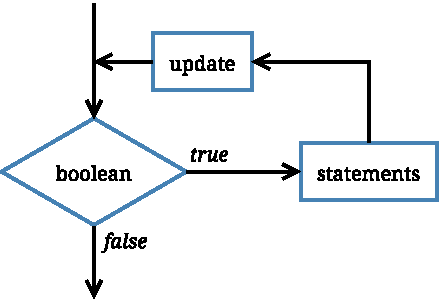
\includegraphics[height=10em]{for.pdf}
\end{minipage}


\quest{10 min}


\Q Identify the components of each \java{for} loop.

\begin{multicols}{2}

\textbf{Loop A:}

\begin{enumerate}
\item initialize \ans[5em]{\jans{i = 1}}
\item test       \ans[5em]{\jans{i <= 10}}
\item update     \ans[5em]{\jans{i++}}
\end{enumerate}

\columnbreak

\textbf{Loop B:}

\begin{enumerate}
\item initialize \ans[5em]{\jans{i = 10}}
\item test       \ans[5em]{\jans{i >= 1}}
\item update     \ans[5em]{\jans{i--}}
\end{enumerate}

\end{multicols}


\newpage


\Q Rewrite each \java{for} loop as a \java{while} loop.

\begin{multicols}{2}

\textbf{Loop A:}

\begin{answer}[6em]
\begin{javaans}
i = 1;
while (i <= 10) {
    System.out.println(i);
    i++;
}
\end{javaans}
\end{answer}

\columnbreak

\textbf{Loop B:}

\begin{answer}[6em]
\begin{javaans}
i = 10;
while (i >= 1) {
    System.out.println(i);
    i--;
}
\end{javaans}
\end{answer}

\end{multicols}


\Q What do each of the \java{for} loops output to the screen? Be specific.

\begin{answer}
The first loop prints the numbers 1 to 10, and the second loop prints the numbers 10 to 1.
Each number is on its own line.
\end{answer}


\Q \label{loophead}
Describe how to change the \java{for} loops to print even numbers only (i.e., the output should be 2 4 6 8 10 and 10 8 6 4 2).

\begin{answer}
Change loop A to:~ \jans{for (i = 2; i <= 10; i += 2)}

\medskip
Change loop B to:~ \jans{for (i = 10; i >= 2; i -= 2)}
\end{answer}


\Q In mathematics, the factorial of an integer $n$ (denoted by $n!$) is the product of all positive integers less than or equal to $n$.
For example, the factorial of 5 is:

\begin{quote}
$5! = 5 * 4 * 3 * 2 * 1 = 120$
\end{quote}

The following code computes the factorial of 5:

\begin{quote}
\begin{javalst}
fact = 1;
i = 5;
while (i > 1) {
    fact *= i;
    i--
}
\end{javalst}
\end{quote}

\begin{enumerate}

\item Rewrite the code above using a \java{for} loop instead of a \java{while} loop.

\begin{answer}[5em]
\begin{javaans}
fact = 1;
for (i = 5; i > 1; i--) {
    fact *= i;
}
\end{javaans}
\end{answer}

\item How would you change the code to compute the factorial of 12?

\begin{answer}[2em]
Simply change ~\java{i = 5} ~to ~\java{i = 12}.
\end{answer}

\end{enumerate}
